\subsection{Постановка задачи на разработку программы}
    Цель работы - составить и реализовать алгоритм глобального распределения регистров в эмуляторе QEMU.

\bigskip
Задачи работы:

\smallskip
\begin{my_enumerate}
\item Изменение алгоритма анализа жизни переменных.
\item Определение наиболее подходящих переменных для помещения на регистры.
\item Изменение логики сохранения регистров в память.
\item Изменение логики поиска свободных регистров и освобождения регистров.
\item Изменение логики работы аллокатора регистров.
\item Внедрение дополнительного прохода по массиву инструкций для определения точек сохранения и загрузки переменных в регистры.
\end{my_enumerate}


\subsection{Описание алгоритма и функционирования программы}


%=============================================================
\subsubsection{Выбор алгоритма}

Одной из актуальных задач в области програмной эмуляции является увеличение ее производительности.

Эмулятор QEMU - это полносистемный эмулятор с открытым исходным кодом позволяющий виртуализировать вычислительные системы с процессором, памятью и периферийными устройствами. В часности QEMU позволяет, например, воспроизводить работу программы скомпилированой для архитектуры процессоров ARM на другой архитектуре, например, на х86\_64.

QEMU использует динамическую двоичную трансляцию, компилируя код для исполнения в процессе работы. На данный момент алгоритмы оптимизации, в частности, алгоритм распределения регистров, являются локальными. Они работают только
в пределах одного базового блока.

Данная курсовая работа нацелена на написание алгоритма глобального распределения регистров. Алгоритм должен распределить и назначить регистры переменным внутри одного блока трансляции. Для алгоритм оценивает влияние каждой переменной на производительность (вес переменной). Далее происходит поиск точек программы наиболее подходящих для загрузки переменных на регистры и для сохранения регистров в память относительно производительности работы эмулятора. Более трудоемкие основанные, например, на раскраске графа алгоритмы не подходят для QEMU из\-за высоких затрат на время работы, с другой стороны основанные на линейном сканировании алгоритмы в действительности оказались сложны в реализации так как требовали работы не только самого алгоритма для распределения регистров, но и реализации анализа достигающих определений.

Для оценки веса переменной используется один из наиболее простых способов. Оценивается частота встречаемости переменной в качестве входного или выходного параметра в инструкциях текущего блока трансляции.

При поиске точек программы для загрузки и сохранения переменных в регистры необходимо учитывать ограничения инструкций. Некоторые инструкции имеют ограничения по использованию регистров, которые необходимо принимать во внимание. Например, INDEX\_op\_exit\_tb или INDEX\_op\_call, обозначающие выход из блока трансляции или вызов функции требуют чтобы перед их выполнением значения регистров были сохранены в память, а сами регистры были свободны для использования.

Результаты работы алгоритма хранятся в структуре TCGOp, там же где хранятся результаты работы анализа жизни переменных. Таким образом результаты работы алгоритмов доступны аллокатору регистров, который использует информармацию и от анализа жизни переменных, и от алгоритма глобального распределения регистров, для того чтобы выбрать наиболее подходящие с относительно производительности точки для сохранения и загрузки переменных.

Алгоритм глобального распределения регистров работает во время перевода кода из внутреннего представления QEMU в коды команд для основной архитектуры. Алгоритм запускается из функции tcg\_gen\_code файла tcg/tcg.c

\begin{figure}[h!]
    \centering
    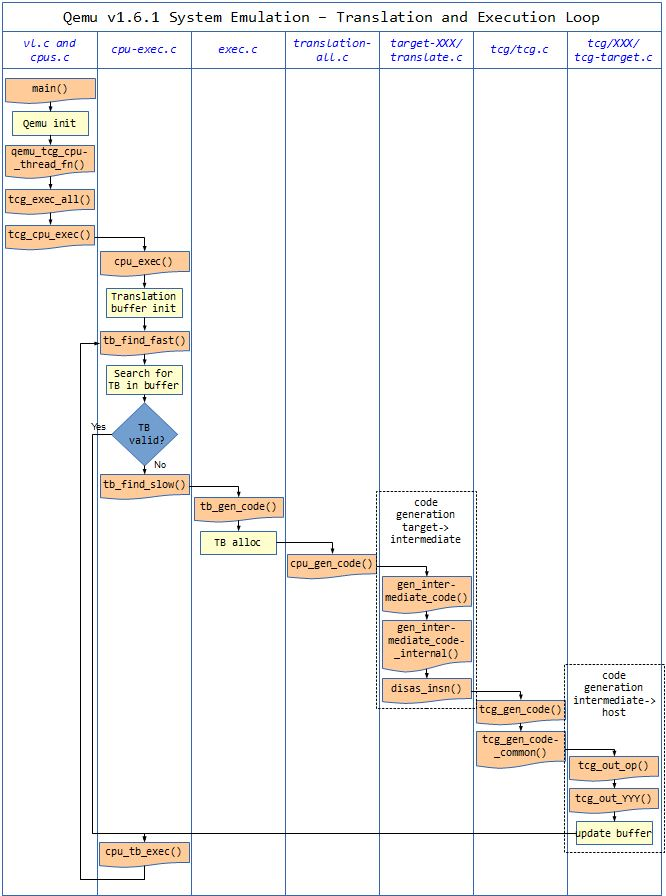
\includegraphics[width=0.9\textwidth]{qemu_graph.jpg}
    \caption{Цикл трансляции и выполнения. Алгоритм распределения регистров запускается из фунцкции tcg\_gen\_code}
\end{figure}

\newpage


При разработке алгоритма необходимо было учесть ограничения инструкций внутреннего представления QEMU, в особенности тех, что влияют на переходы между базовыми блоками и входами/выходами из блоков трансляции. Некоторые инструкции, такие как call в рамках договора о вызове на платформе х86\_64 требуют синхронизировать переменные в регистрах с памятью.

\begin{figure}[h!]
    \centering
    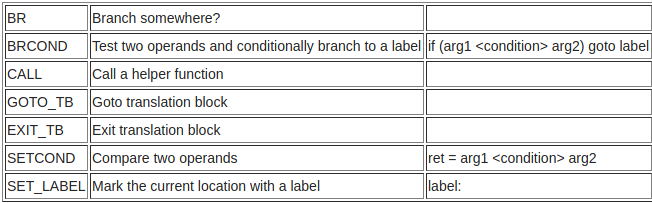
\includegraphics[width=0.8\textwidth]{table_flow.png}
    \caption{Инструкции внутреннего представления QEMU для перехода между блоками}
\end{figure}

%=============================================================
\subsubsection{Основные определения и структуры данных}

Структура ТCGContext используется для хранения информации при генерации кодов команд. Данная структура содержит массив с инструкциями текущего блока трансляции во внутреннем представлении QEMU gen\_op\_buf, аргументы для каждой инструкции содержится в отдельном массиве gen\_opparam\_buf. Ниже приведено ее полное определение:

\begin{small}
\begin{verbatim}
struct TCGContext {
    uint8_t *pool_cur, *pool_end;
    TCGPool *pool_first, *pool_current, *pool_first_large;
    int nb_labels;
    int nb_globals;
    int nb_temps;
    int nb_indirects;

    /* goto_tb support */
    tcg_insn_unit *code_buf;
    uint16_t *tb_jmp_reset_offset; /* tb->jmp_reset_offset */
    uintptr_t *tb_jmp_insn_offset; /* tb->jmp_target_arg if direct_jump */
    uintptr_t *tb_jmp_target_addr; /* tb->jmp_target_arg if !direct_jump */

    TCGRegSet reserved_regs;
    intptr_t current_frame_offset;
    intptr_t frame_start;
    intptr_t frame_end;
    TCGTemp *frame_temp;

    tcg_insn_unit *code_ptr;

    // choose a temporary (local temp or global) to be placed on the register and kept there
    GAVar drag_through[REGS_FOR_GLOBAL_ALLOC];
    int drag_through_len;
    int exits_count;

#ifdef CONFIG_PROFILER
    /* profiling info */
    int64_t tb_count1;
    int64_t tb_count;
    int64_t op_count; /* total insn count */
    int op_count_max; /* max insn per TB */
    int64_t temp_count;
    int temp_count_max;
    int64_t del_op_count;
    int64_t code_in_len;
    int64_t code_out_len;
    int64_t search_out_len;
    int64_t interm_time;
    int64_t code_time;
    int64_t la_time;
    int64_t opt_time;
    int64_t restore_count;
    int64_t restore_time;
#endif

#ifdef CONFIG_DEBUG_TCG
    int temps_in_use;
    int goto_tb_issue_mask;
#endif

    int gen_next_op_idx;
    int gen_next_parm_idx;

    /* Code generation.  Note that we specifically do not use tcg_insn_unit
       here, because there's too much arithmetic throughout that relies
       on addition and subtraction working on bytes.  Rely on the GCC
       extension that allows arithmetic on void*.  */
    void *code_gen_prologue;
    void *code_gen_epilogue;
    void *code_gen_buffer;
    size_t code_gen_buffer_size;
    void *code_gen_ptr;
    void *data_gen_ptr;

    /* Threshold to flush the translated code buffer.  */
    void *code_gen_highwater;

    TBContext tb_ctx;

    /* Track which vCPU triggers events */
    CPUState *cpu;                      /* *_trans */
    TCGv_env tcg_env;                   /* *_exec  */

    /* These structures are private to tcg-target.inc.c.  */
#ifdef TCG_TARGET_NEED_LDST_LABELS
    struct TCGLabelQemuLdst *ldst_labels;
#endif
#ifdef TCG_TARGET_NEED_POOL_LABELS
    struct TCGLabelPoolData *pool_labels;
#endif

    TCGTempSet free_temps[TCG_TYPE_COUNT * 2];
    TCGTemp temps[TCG_MAX_TEMPS]; /* globals first, temps after */

    /* Tells which temporary holds a given register.
       It does not take into account fixed registers */
    TCGTemp *reg_to_temp[TCG_TARGET_NB_REGS];

    TCGOp gen_op_buf[OPC_BUF_SIZE];
    TCGArg gen_opparam_buf[OPPARAM_BUF_SIZE];

    uint16_t gen_insn_end_off[TCG_MAX_INSNS];
    target_ulong gen_insn_data[TCG_MAX_INSNS][TARGET_INSN_START_WORDS];
};
\end{verbatim}
\end{small}


Структура TCGOp хранит в себе информацию об инструкции, о ее параметрах и типе. В ней содержится информация полученная в ходе работы алгоритма для анализа жизни переменных и информация полученная в ходе работы
алгоритма глобального распределения регистров. В частности результаты анализа жизни переменных используются чтобы подсказать аллокатору регистров, что переменная больше не используется в данном базовом блоке, а результаты алгоритма по глобальному распределению регистров используются для того чтобы подсказать аллокатору регистров, когда переменную стоит протащить в следующий базовый блок, а когда их стоит сохранить в память и освободить регистры.

\begin{small}
\begin{verbatim}
typedef struct TCGOp {
    TCGOpcode opc   : 8;        /*  8 */

    /* Index of the prev/next op, or 0 for the end of the list.  */
    unsigned prev   : 10;       /* 18 */
    unsigned next   : 10;       /* 28 */

    /* The number of out and in parameter for a call.  */
    unsigned calli  : 4;        /* 32 */
    unsigned callo  : 2;        /* 34 */

    /* Index of the arguments for this op, or 0 for zero-operand ops.  */
    unsigned args   : 14;       /* 48 */

    /* Lifetime data of the operands. */
    unsigned life   : 16;       /* 64 */

    bool ga_pre_load_regs;
    bool ga_post_load_regs;
    bool ga_sync_regs;
    bool ga_free_regs;
} TCGOp;
\end{verbatim}
\end{small}


\textbf{Структура}
GAVar (Global Allocator Variable) используется на этапе оценки веса переменных. Осуществляется проход по массиву инструкций, подчитывается какие переменных наиболее часто выступают в роли входных или выходных параметров. Эта информация храниться в массиве структур GAVar.

\begin{small}
\begin{verbatim}
typedef struct GAVar {
#ifdef CONFIG_DEBUG_TCG
    char* name;           //< name of variable as assigned by QEMU
#endif
    int count;            //< weight of var
    TCGTemp *ts;          //< pointer to actual temp
} GAVar;
\end{verbatim}
\end{small}


В QEMU есть набор инструкций внутреннего представления для записи и чтения памяти. Они приведены ниже. Однако в связи с тем что алгоритм распределения регистров работает только с глобальными переменными для загрузки переменной на регистр и для сохранения ее в память использовалась команда MOV.

\begin{figure}[h!]
    \centering
    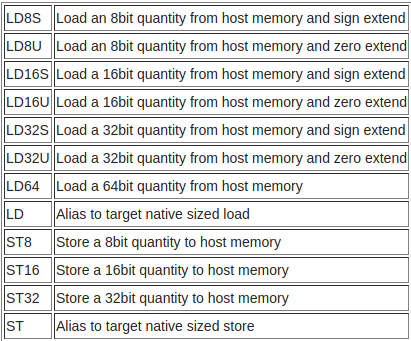
\includegraphics[width=0.8\textwidth]{table_load_store.png}
    \caption{Инструкции внутреннего представления QEMU для чтения и записи памяти}
\end{figure}



%=============================================================
\subsubsection{Описание алгоритма}

Первым этапом работы алгоритма является запуск алгоритма для анализа жизни переменных. Анализ жизни переменных
используется для того чтобы снизить количество одновременно используемых регистров. Если становится понятно, что аргумент операции далее в базовом блоке не используется, алгоритм анализа жизни переменных помечает аргумент либо как кандидата на синхронизацию, в случае если это глобальная или локальная переменная, либо как мертвого в случае если это простая переменная или константа.

Определение веса переменных осуществляется в процессе прохода по массиву инструкций текущего блока трансляции и подсчета количества использований для каждой из глобальных переменных. Внутреннее представление QEMU различает несколько типов переменных: переменные, глобальные переменные, локальные переменные и константы. Простые переменные существуют только внутри базового блока, их значение не используется после выхода из блока. Локальные переменные мало используются в текущей реализации QEMU. Алгоритм глобального распределения регистров рассматривает только глобальные переменные.

После просмотра всех параметров для всех инструкций данного блока трансляции и подсчета веса для каждой переменной, выбираются несколько самых часто встречаемых переменных. Ниже приведен фрагмент кода для выбора нескольких самых весомых переменных:

\begin{small}
\begin{verbatim}
    // for each variable
    for (int i=0; i < metas_len; i++) {

        // find current smallest occurence in drag_through
        int min_known_idx = 0;

        for (int k=0; k < REGS_FOR_GLOBAL_ALLOC; k++) {
            if (s->drag_through[k].count < s->drag_through[min_known_idx].count) {
                min_known_idx = k;
            }
        }
        
        // check if current var is larger
        if (metas[i].count > s->drag_through[min_known_idx].count) {
            s->drag_through[min_known_idx] = metas[i];
        }
        
    }

    // choose whichever is smaller
    s->drag_through_len = (metas_len < REGS_FOR_GLOBAL_ALLOC) ? metas_len : REGS_FOR_GLOBAL_ALLOC;
\end{verbatim}
\end{small}


Следующим шагом  является определение тех инструкций когда переменные должны занять регистры и когда они должны их освободить. Для этого производится еще один проход по массиву инструкций текущего блока трансляции и с учетом контекста и внутреннего состояния операции помечаются флагами. Упрощенный фрагмент кода отвечающий за расставление флагов приведен ниже:

\begin{small}
\begin{verbatim}
    for (oi = s->gen_op_buf[0].next; oi != 0; oi = oi_next) {
        TCGOp * const op = &s->gen_op_buf[oi];
        TCGOpcode opc = op->opc;
        const TCGOpDef *def = &tcg_op_defs[opc];
        TCGArg * const args = &s->gen_opparam_buf[op->args];

        oi_next = op->next;

        switch (opc) {
        case INDEX_op_insn_start:
            if (! has_global_reg_alloc_init) {
                has_global_reg_alloc_init = true;
                op->ga_pre_load_regs = true;
            }
            break;
        case INDEX_op_set_label:
            if (arg_label(args[0]) == early_exit_label) {
                dont_spill_on_next_exit_tb = true;
            }
            break;
        case INDEX_op_call:
            // before the call must sync and free regs
            op->ga_sync_regs = true;
            op->ga_free_regs = true;
            op->ga_post_load_regs = true;
            break;
        }
    }
\end{verbatim}
\end{small}

После этого контроль переходит непосредственно к механизму аллокации регистров, который основываясь на работе анализа жизни переменных и алгоритма глобального распределения регистров решает когда и какую переменную поместить из памяти на регистр, а когда поместить обратно в память. Собственно механизм аллокации регистров также занимается и  вызовом функций для генерации кодов команд.


\subsection{Mетод организации входных и выходных данных}

\subsubsection{Описание метода входных и выходных данных}
Входными данными для работы алгоритма является массив инструкций для блока трансляции в формате внутреннего представления эмулятора QEMU. Для работы алгоритма необходима исполняемая программа, которая может быть запущена в эмуляторе QEMU. Входной файл исполняемой программы может быть создан в любой среде разработки на платформе которую поддерживает эмулятор QEMU, например, х86\_64 с операционной системой Linux.

\begin{my_enumerate}
\item Файл программы должен представлять собой исполняемый файл предназначенный для запуска в userspace операционной системы Linux на архитектуре х86\_64.
\item Файл программы должен быть предоставлен в формате ELF.
\end{my_enumerate}

\medskip
Выходными данными для алгоритма являются коды команд для архитектуры х86\_64.



\subsection{Выбор состава технических средств}

\subsubsection{Состав технических и програмных средств}

Для работы алгоритма в эмуляторе QEMU необходимо учесть следующие системные требования:
\begin{my_enumerate}
\item Компьютер, оснащенный:
    \begin{my_enumerate}
    \item 64-разрядный (x86\_64) процессор с тактовой частотой 1 гигагерц (ГГц) или выше;
    \item 2 ГБ оперативной памяти (ОЗУ);
    \item 1.5 ГБ свободного места на жестком диске;
    \end{my_enumerate}
\item Монитор
\item Мышь
\item Клавиатура
\end{my_enumerate}
